\documentclass[11pt,a4paper]{article}

\usepackage[T1]{fontenc}
\usepackage[margin=2.3cm]{geometry}
\usepackage{amsmath,amssymb}
\usepackage{booktabs}
\usepackage{array}
\usepackage{enumitem}
\usepackage{graphicx}
\usepackage{tikz}
\usetikzlibrary{arrows.meta,positioning,patterns}
\usepackage[most]{tcolorbox}
\usepackage[hidelinks]{hyperref}
\usepackage{parskip}

\graphicspath{{../figures/}}
\setlist{itemsep=2pt,topsep=3pt}
\renewcommand{\arraystretch}{1.25}

\newtcolorbox{keybox}[1][]{colback=gray!10,colframe=black!60,boxrule=0.5pt,arc=2pt,left=6pt,right=6pt,top=4pt,bottom=4pt,#1}
\newtcolorbox{saybox}[1][]{colback=white,colframe=black!40,boxrule=0.5pt,arc=2pt,left=6pt,right=6pt,top=4pt,bottom=4pt,fonttitle=\bfseries,title={#1}}

\title{\textbf{Understanding Our Methodology}\\[4pt]
\large A plain-language guide to the contributions, the method and the experimental design of\\ \emph{Change-Characteristic-Aware Window Selection for Unsupervised Concept Drift Detection in Real-Time Text Streams}}
\author{Explanation guide for the group}
\date{}

\begin{document}
\maketitle

\begin{keybox}
\textbf{How to use this guide.} This guide follows the report \texttt{midterm\_report\_methodology.tex} section by section. Part~\ref{sec:words} explains the few words you need first. Part~\ref{sec:contrib} explains the three contributions. Parts~\ref{sec:method} and \ref{sec:exp} go through every subsection of the Methodology and Experimental Design, including every figure, equation and the algorithm. Each part ends with a box that tells you what to \emph{say} when you present it. Part~\ref{sec:qa} lists questions the faculty may ask, and Part~\ref{sec:script} is a short script for explaining the whole method.
\end{keybox}

\tableofcontents
\newpage

%====================================================================
\section{The Story in One Paragraph}

Text keeps arriving: news articles, forum posts, product reviews. Over time the \emph{topics} change. A model trained on old text slowly becomes outdated. We want a small program, a \emph{drift detector}, that watches the stream and rings an alarm when the text has really changed, so that the model can be updated. The difficulty is that we have \textbf{no labels}, so the detector must decide only by looking at the text itself. Our detector is built on an existing method called ADWIN-U. ADWIN-U keeps a ``memory window'' of recent data and throws away the old part of the window as soon as it is sure something changed. Our idea is to make this decision smarter: when the evidence of change is strong we act at once, when it is weak we \emph{wait and watch}, and if the weak evidence keeps coming back we throw away \emph{only part} of the old data.

%====================================================================
\section{Words You Need First}
\label{sec:words}

\begin{description}[leftmargin=0pt]
\item[Data stream.] Data that arrives one item at a time and never stops. We cannot store everything, so we look at each item once.
\item[Concept drift.] The data changes its behaviour over time. In our case, the topics of the text change. Example: a news feed suddenly has many more articles about an election.
\item[Label.] The correct answer for an item, for example ``this article is about sports''. Labels need a human, so in real streams they are usually missing. Our detector never uses labels.
\item[Embedding.] A list of numbers that represents the meaning of a text. We use 384 numbers per document. Texts with similar meaning get similar lists.
\item[Window.] The detector's short-term memory: a summary of the most recent values it has seen.
\item[Cut.] Throwing away the older part of the window, because it no longer looks like the new data.
\item[ADWIN.] A well-known detector (2007) that keeps a window, splits it into an \emph{older} part and a \emph{newer} part, and compares their averages. If they differ by more than a safe threshold, it cuts the older part and raises an alarm.
\item[ADWIN-U.] A 2025 version of ADWIN that needs no labels. Instead of watching a classifier's mistakes, it watches a simple number computed from each example (such as skewness or kurtosis). This is our starting point.
\item[False alarm.] An alarm when nothing really changed.
\item[Detection delay.] How long after a real change the alarm comes.
\end{description}

%====================================================================
\section{The Three Contributions}
\label{sec:contrib}

The report lists three contributions. Here is what each one means.

\subsection*{Contribution (i): a label-free window-selection policy with a hold state and a graded cut}

\textbf{What the report says.} We propose a label-free window-selection policy with a hold state and a graded cut that contains ADWIN-U as a special case at the same $O(\log W)$ cost.

\textbf{In plain words.} ADWIN-U has only two choices after each check: do nothing, or throw away the whole old part of the window. We give the detector more choices:
\begin{itemize}
\item \textbf{Full cut} when the evidence is strong (same as ADWIN-U).
\item \textbf{Hold} when the evidence is weak: do not cut yet, raise a warning and keep watching.
\item \textbf{Graded cut} when the weak evidence keeps pointing the same way for several checks: throw away only the \emph{oldest} part of the old data. The stronger the evidence, the more we throw away.
\end{itemize}

\textbf{An everyday picture.} Think of a doctor watching a patient's temperature. A very high reading means act now (full cut). A slightly high reading once means nothing yet, just keep an eye on it (hold). Slightly high readings for three days in a row mean something is going on, so start a mild treatment (graded cut).

\textbf{``Contains ADWIN-U as a special case''} means that if we set our two thresholds to the same value, our method behaves exactly like ADWIN-U. So our method is an extension, not a replacement, and any difference in results comes from what we added.

\textbf{``At the same $O(\log W)$ cost''} means it should be just as fast and use just as little memory as ADWIN-U. We only add one counter and one sign. We will measure this to confirm it.

\subsection*{Contribution (ii): lower delay on gradual and subtle drift}

\textbf{What the report says.} We show that graded cutting lowers detection delay on gradual and subtle drift at a matched false-alarm rate, while abrupt drift is handled as in ADWIN-U.

\textbf{In plain words.} Some changes are sudden (abrupt), like switching from sports news to political news overnight. Others are slow (gradual) or small (subtle), like sports news slowly turning into more basketball and less football. Slow and small changes produce only weak evidence, so ADWIN-U waits a long time before it is ``sure'' enough to act. Our hold and graded cut can react to weak but \emph{repeated} evidence, so we expect to catch these changes earlier.

\textbf{``At a matched false-alarm rate''} is important. Any detector can be made faster by making it more nervous, but then it also gives more false alarms. To be fair, we first tune every detector so they all give the \emph{same} number of false alarms on data with no change. Only then do we compare delays.

\textbf{``Abrupt drift is handled as in ADWIN-U''} means that for sudden changes the evidence is strong, so our method does a full cut, which is exactly what ADWIN-U does. We do not claim to beat ADWIN-U there.

\textbf{Note.} This is what we \emph{expect} and plan to test. It is a hypothesis until the experiments are done.

\subsection*{Contribution (iii): do ADWIN-U's statistics work on text?}

\textbf{What the report says.} We examine whether ADWIN-U's per-instance statistics capture topic drift in sentence embeddings, compared with a centroid-distance signal.

\textbf{In plain words.} ADWIN-U turns each example into one number, such as skewness (how lopsided the values are) or kurtosis (how extreme the values are). This worked well on sensor data. But for text, a change of topic might not change the \emph{shape} of the 384 numbers at all, only \emph{which} numbers are large. So we test whether these statistics notice topic changes. As a backup we also use a second number that is closer to meaning: how far each new document is from the ``average document'' seen so far (the centroid distance).

\textbf{Why it matters.} If the statistics do not react to topic drift, no window policy can help, because the detector would be blind. So this check comes first.

\begin{saybox}{What to say}
``Our main contribution is the rule that decides \emph{how much} of the window to throw away after seeing evidence of change: a full cut for strong evidence, a hold for weak evidence and a graded cut when weak evidence persists. We expect this to catch slow and small changes earlier at the same false-alarm rate. We also check whether ADWIN-U's simple statistics even work for text.''
\end{saybox}

%====================================================================
\section{Methodology, Subsection by Subsection}
\label{sec:method}

\subsection{The framework figure (Fig.~2 in the report)}

\begin{figure}[h]
\centering
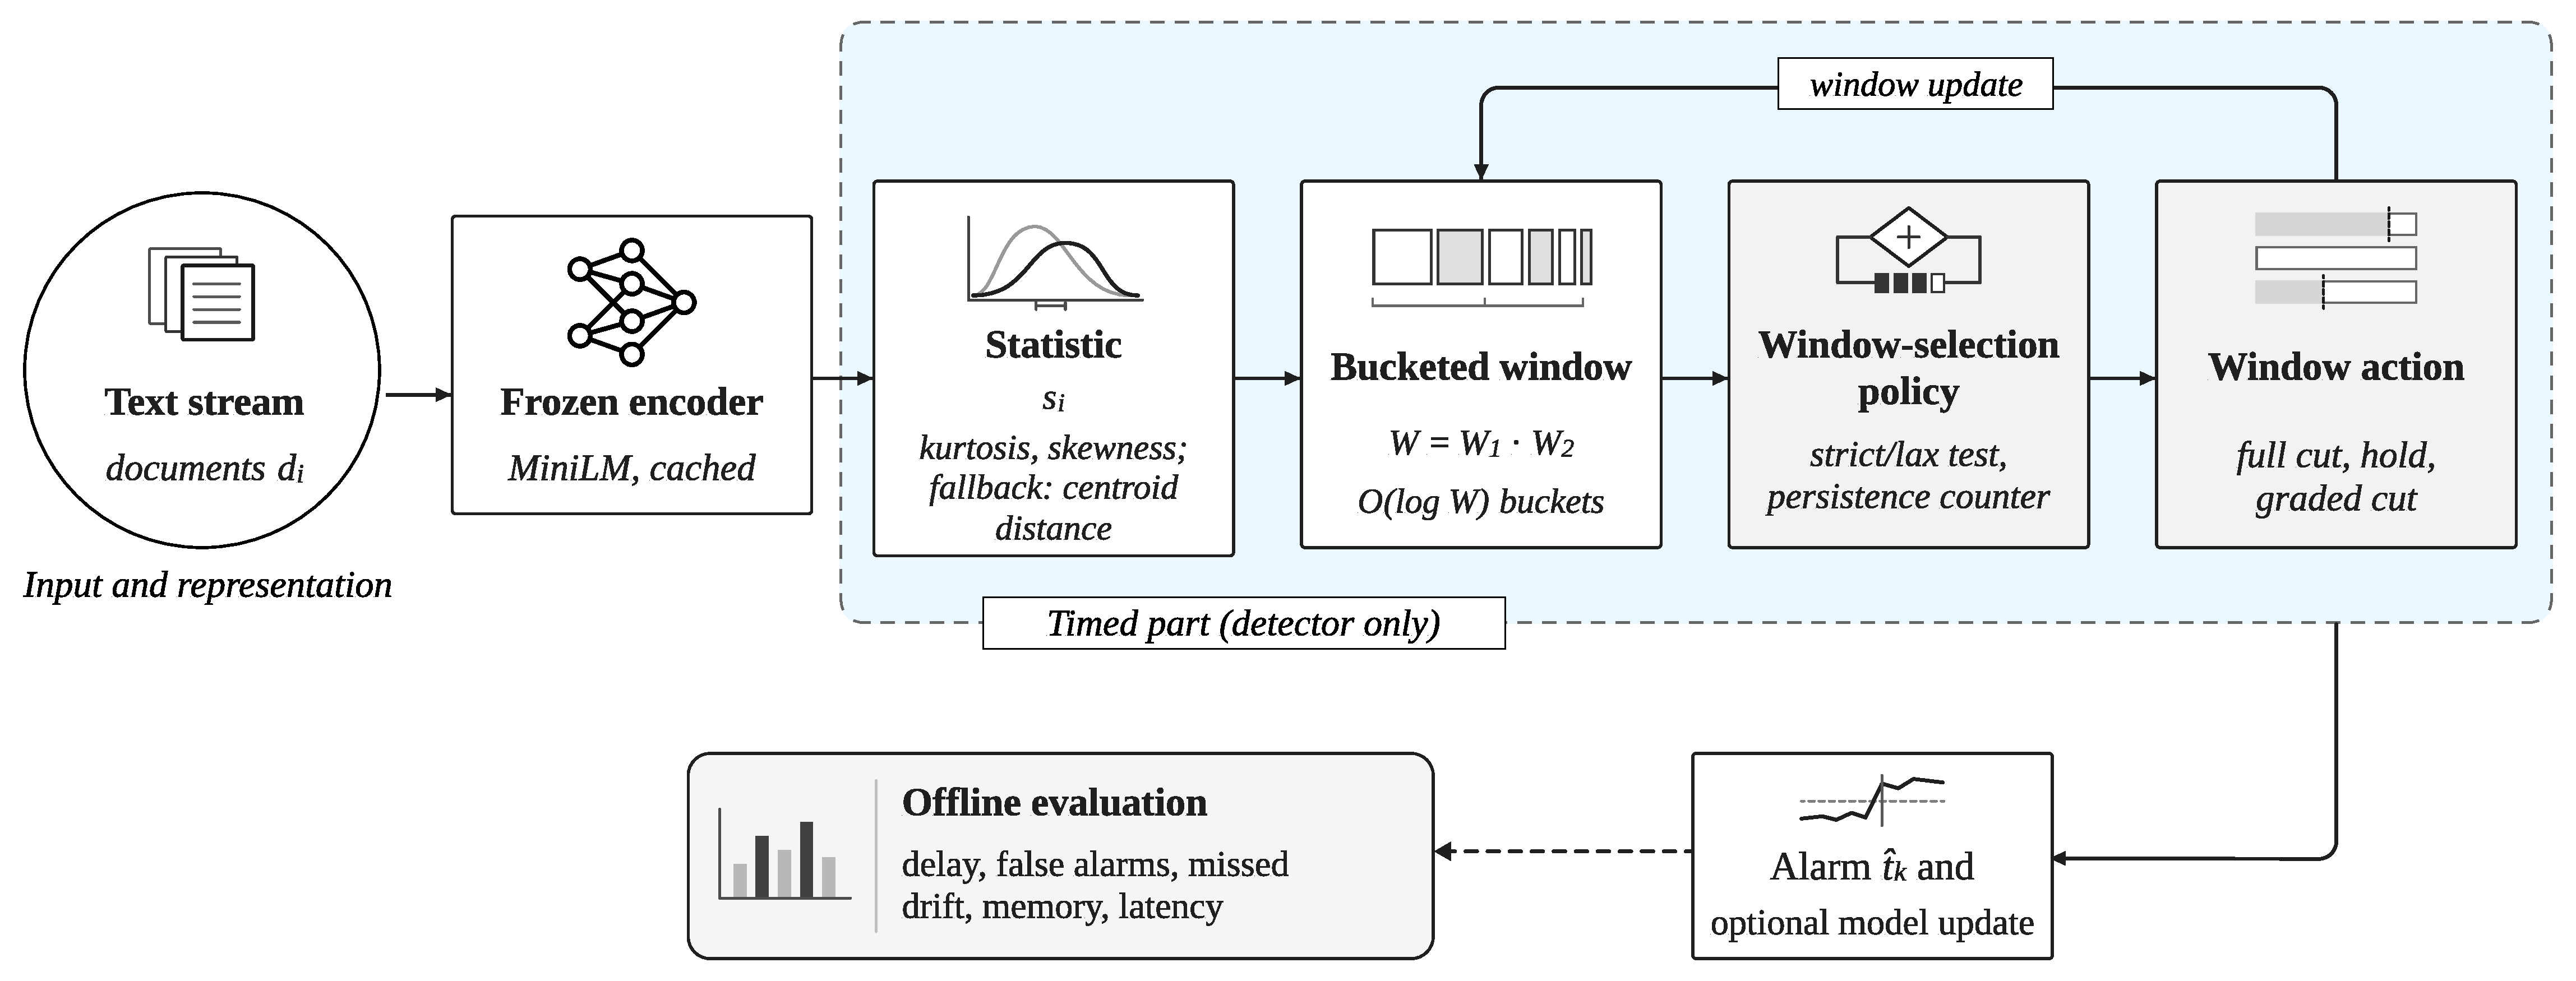
\includegraphics[width=\linewidth]{pipeline.pdf}
\caption{The framework figure from the report.}
\end{figure}

Read the figure from left to right like a factory line.
\begin{enumerate}
\item \textbf{Text stream (circle).} Documents $d_1, d_2, \dots$ arrive one by one.
\item \textbf{Frozen encoder.} A ready-made language model (MiniLM) turns each document into 384 numbers. ``Frozen'' means we never retrain it. ``Cached'' means we compute the numbers once and save them.
\item \textbf{Statistic $s_i$.} Each list of 384 numbers is squeezed into \emph{one} number: kurtosis or skewness, or the centroid distance as a backup.
\item \textbf{Bucketed window.} The detector's memory. It stores the numbers in a compressed form (buckets) and is split into an older part $W_1$ and a newer part $W_2$.
\item \textbf{Window-selection policy (shaded).} Our new part. It looks at how different $W_1$ and $W_2$ are and decides what to do.
\item \textbf{Window action (shaded).} Full cut, hold or graded cut. The ``window update'' arrow going back shows that the action changes the window.
\item \textbf{Alarm and optional model update.} If there was a cut, an alarm is raised and the user may retrain their model.
\item \textbf{Offline evaluation.} Afterwards we measure delay, false alarms, missed drift, memory and speed.
\end{enumerate}
The \textbf{dashed blue box} (``Timed part'') shows which parts we time. The encoder is outside it, so our speed measurements are about the detector only. The \textbf{shaded boxes} are what is new in our work.

\subsection{Problem formulation (III-A)}

This subsection says precisely what the detector gets and what it must produce.
\begin{itemize}
\item \textbf{Input:} a never-ending sequence of documents $S=(d_1,d_2,\dots)$. Each one becomes an embedding $x_i=f(d_i)$, a list of $D=384$ numbers.
\item \textbf{Hidden truth:} somewhere in the stream there are drift points $t_1, t_2, \dots$ where the data changes. The detector does not know them.
\item \textbf{Output:} a list of alarm times $\hat t_1, \hat t_2, \dots$, the moments when the detector thinks a change happened. (The hat symbol $\hat{\ }$ means ``our guess''.)
\item \textbf{Rules:} look at each document only once, never use a label, keep only a small summary of the past.
\item \textbf{Goals:} alarm soon after each real change, few alarms when nothing changes, miss nothing, and be fast and light.
\end{itemize}
Labels are used only by us, the researchers, to build test streams where we know where the changes are.

\subsection{Framework overview (III-B)}

This is the same four-stage line as the figure: (1) encode and cache, (2) compute one number per document, (3) put it into the window, (4) let the policy decide. Stages 2 to 4 are the detector and are timed. Stages 2 and 3 come from ADWIN-U. Stage 4 is ours.

\subsection{Text representation and drift signal (III-C)}

\subsubsection*{Encoder}
We use the model \texttt{all-MiniLM-L6-v2}, a small and fast version of Sentence-BERT. It outputs 384 numbers per document. Because we never retrain it, any change the detector sees comes from the text, not from the model changing.

\subsubsection*{Per-instance statistic (Eq.~1)}
For one document, take its 384 numbers. First standardize them: subtract their average $\bar x_i$ and divide by their spread $\sigma_i$. This gives $z_{ij}$. Then
\[
s_i^{\mathrm{kurt}}=\frac{1}{D}\sum_{j=1}^{D}z_{ij}^{4},\qquad s_i^{\mathrm{skew}}=\frac{1}{D}\sum_{j=1}^{D}z_{ij}^{3}.
\]
\begin{itemize}
\item \textbf{Skewness} (power 3) tells us whether the numbers lean to one side. Zero means balanced.
\item \textbf{Kurtosis} (power 4) tells us whether there are a few very extreme numbers. Raising to the 4th power makes extreme values dominate. A normal bell curve gives about 3.
\end{itemize}
So each document becomes one number. These are the same formulas ADWIN-U uses. The worry, which we test, is that a change of topic may move \emph{which} of the 384 numbers are large without changing the overall shape, so these statistics might not notice.

\subsubsection*{Centroid-distance signal (Eq.~2)}
The \emph{centroid} $c_i$ is the average embedding of all documents seen since the last alarm, like the ``typical document'' so far. For each new document we measure how far its direction is from the centroid:
\[
s_i^{\mathrm{cos}} = 1-\cos(\text{angle between } x_i \text{ and } c_i).
\]
If the document points the same way as the centroid, the value is 0. If it is unrelated (at a right angle), the value is 1. When the topic changes, new documents point away from the old centroid, so these values go up on average. This is the standard way to compare Sentence-BERT embeddings.

\subsubsection*{Scaling}
The threshold used later assumes every value lies between 0 and 1. Kurtosis, for example, does not. So we watch the first few hundred values (a ``warm-up''), note the smallest and largest, and rescale everything into $[0,1]$. Values outside the range are clipped.

\emph{Example.} Warm-up minimum 2.1, maximum 4.5. A later value 3.3 becomes $(3.3-2.1)/(4.5-2.1)=0.5$. A value 5.0 would be above the maximum, so it is clipped to 1.

\subsection{Adaptive window and change test (III-D)}

This subsection explains how ADWIN decides that something changed. We keep this part unchanged.

\textbf{The window.} The scaled numbers go into the window $W$. To save memory, old values are merged into buckets of size 1, 2, 4, 8, \dots, so a window of a million values needs only a few dozen buckets. That is why memory and time grow only like $\log|W|$.

\textbf{The split.} Every $\tau$ new values, the detector tries splitting the window at each bucket boundary into an older part $W_1$ (size $n_1$) and a newer part $W_2$ (size $n_2$). For each split it computes the \textbf{gap} between their averages (Eq.~3):
\[
g=\hat\mu_{W_1}-\hat\mu_{W_2}.
\]
If nothing changed, both parts have about the same average and $g$ is close to 0. The sign of $g$ tells us the direction of the change.

\textbf{The threshold (Eq.~4).} How big must $|g|$ be before we believe it? ADWIN uses a formula from Hoeffding's inequality, a classic result that limits how far an average can wander by pure chance:
\[
\varepsilon(\delta)=\sqrt{\frac{1}{2m}\ln\frac{4|W|}{\delta}},\qquad m=\frac{1}{1/n_1+1/n_2}.
\]
You only need to know three things about it:
\begin{itemize}
\item $\delta$ is the \textbf{confidence level}. A smaller $\delta$ makes the threshold bigger, so the test is stricter and gives fewer false alarms.
\item $m$ is the \textbf{harmonic mean} of the two part sizes. More data gives a bigger $m$ and a smaller threshold, because averages over more data are more reliable.
\item If $|g|\ge\varepsilon$, ADWIN and ADWIN-U drop \emph{all} of $W_1$. This single all-or-nothing decision is what our policy replaces.
\end{itemize}

\emph{Example.} With $n_1=n_2=500$ (so $|W|=1000$, $m=250$) and $\delta=0.002$: $\varepsilon=\sqrt{\ln(2{,}000{,}000)/500}=\sqrt{14.51/500}\approx0.170$. So the two averages must differ by at least 0.17 on the $[0,1]$ scale.

\subsection{Window-selection policy (III-E): our contribution}

\subsubsection*{The cut figure (Fig.~3 in the report)}

\begin{figure}[h]
\centering
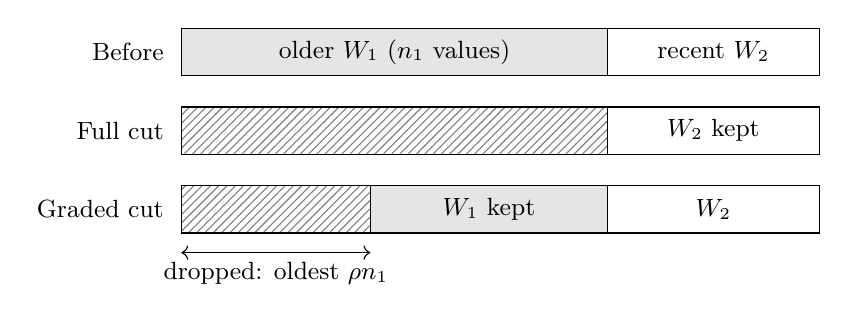
\begin{tikzpicture}[
  seg/.style={draw, minimum height=6mm, inner sep=0pt, font=\small},
  lab/.style={font=\small, anchor=east}
]
\def\a{5.4} \def\b{2.7} \def\d{2.4} \pgfmathsetmacro{\r}{\a-\d}
\node[lab] at (0,0) {Before};
\node[seg, minimum width=\a cm, fill=gray!20, anchor=west] at (0.1,0) {older $W_1$ ($n_1$ values)};
\node[seg, minimum width=\b cm, fill=white, anchor=west] at (\a+0.1,0) {recent $W_2$};
\node[lab] at (0,-1.0) {Full cut};
\node[seg, minimum width=\a cm, pattern=north east lines, pattern color=black!50, anchor=west] at (0.1,-1.0) {};
\node[seg, minimum width=\b cm, fill=white, anchor=west] at (\a+0.1,-1.0) {$W_2$ kept};
\node[lab] at (0,-2.0) {Graded cut};
\node[seg, minimum width=\d cm, pattern=north east lines, pattern color=black!50, anchor=west] at (0.1,-2.0) {};
\node[seg, minimum width=\r cm, fill=gray!20, anchor=west] at (\d+0.1,-2.0) {$W_1$ kept};
\node[seg, minimum width=\b cm, fill=white, anchor=west] at (\a+0.1,-2.0) {$W_2$};
\draw[<->, thin] (0.1,-2.55) -- node[font=\small, below] {dropped: oldest $\rho n_1$} (\d+0.1,-2.55);
\end{tikzpicture}
\caption{Redrawn cut figure. Time runs from left (old) to right (new). Hatched means thrown away.}
\end{figure}

\begin{itemize}
\item \textbf{Before:} the window has an older part (grey) and a recent part (white).
\item \textbf{Full cut:} the whole older part is thrown away (hatched). Only recent data remain. This is what ADWIN-U always does.
\item \textbf{Graded cut:} only the \emph{oldest} slice of the older part is thrown away. Its length is a fraction $\rho$ of $W_1$. The rest of $W_1$ is kept.
\end{itemize}
Why throw away the oldest slice? Because it is the most out of date. Why keep the rest? Because if the change is small, those values are still useful.

\subsubsection*{Two-level test (Eq.~5)}
Instead of one threshold we compute two, using Eq.~4 twice:
\begin{itemize}
\item a \textbf{strict} threshold $\varepsilon_s$ with a small $\delta_s$ (high bar), and
\item a \textbf{relaxed} threshold $\varepsilon_w$ with a larger $\delta_w$ (lower bar).
\end{itemize}
Then every check falls into one of three zones:

\begin{center}
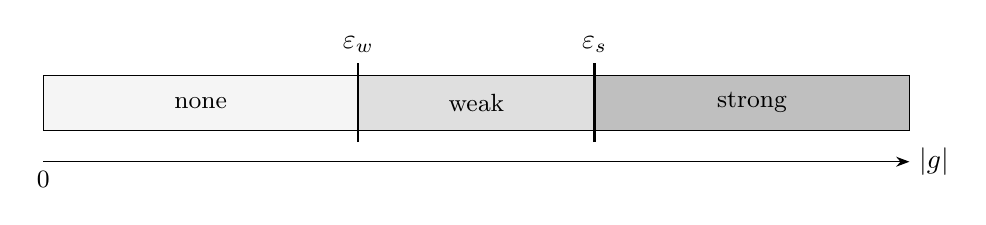
\begin{tikzpicture}
\fill[gray!8] (0,0) rectangle (4,0.7);
\fill[gray!25] (4,0) rectangle (7,0.7);
\fill[gray!50] (7,0) rectangle (11,0.7);
\draw (0,0) rectangle (11,0.7);
\node at (2,0.35) {\small none};
\node at (5.5,0.35) {\small weak};
\node at (9,0.35) {\small strong};
\draw[thick] (4,-0.15) -- (4,0.85) node[above] {$\varepsilon_w$};
\draw[thick] (7,-0.15) -- (7,0.85) node[above] {$\varepsilon_s$};
\draw[-{Stealth}] (0,-0.4) -- (11,-0.4) node[right] {$|g|$};
\node[below] at (0,-0.4) {\small 0};
\end{tikzpicture}
\end{center}

\begin{itemize}
\item \textbf{None} ($|g|<\varepsilon_w$): nothing interesting.
\item \textbf{Weak} ($\varepsilon_w\le|g|<\varepsilon_s$): maybe a change, not sure yet.
\item \textbf{Strong} ($|g|\ge\varepsilon_s$): clearly a change. Full cut and alarm, exactly as ADWIN-U.
\end{itemize}
If several splits are possible, we use the one whose gap is largest compared with its strict threshold, that is, the most convincing split.

\emph{Example.} Same window as before. With $\delta_s=0.002$ we got $\varepsilon_s\approx0.170$. With, say, $\delta_w=0.05$ we get $\varepsilon_w=\sqrt{\ln(80{,}000)/500}\approx0.150$. A gap of 0.16 is in the weak zone. A gap of 0.18 is strong.

\subsubsection*{Hold state and persistence}
When a check is weak, the window is \emph{not} cut. The detector:
\begin{enumerate}
\item enters the \textbf{hold} state and raises a warning (not an alarm),
\item remembers the \textbf{sign} of $g$ (did the average go up or down?),
\item counts with $c$ how many weak checks in a row point the \emph{same} way.
\end{enumerate}
If the evidence disappears or flips direction, the hold is \textbf{released} and $c$ goes back to 0. A real change keeps pushing in one direction, while random noise goes up and down. If $c$ reaches $k$ (for example 3), we believe the change is real and do a graded cut. So one strange reading can never cut the window on its own.

\subsubsection*{The state diagram (Fig.~4 in the report)}

\begin{figure}[h]
\centering
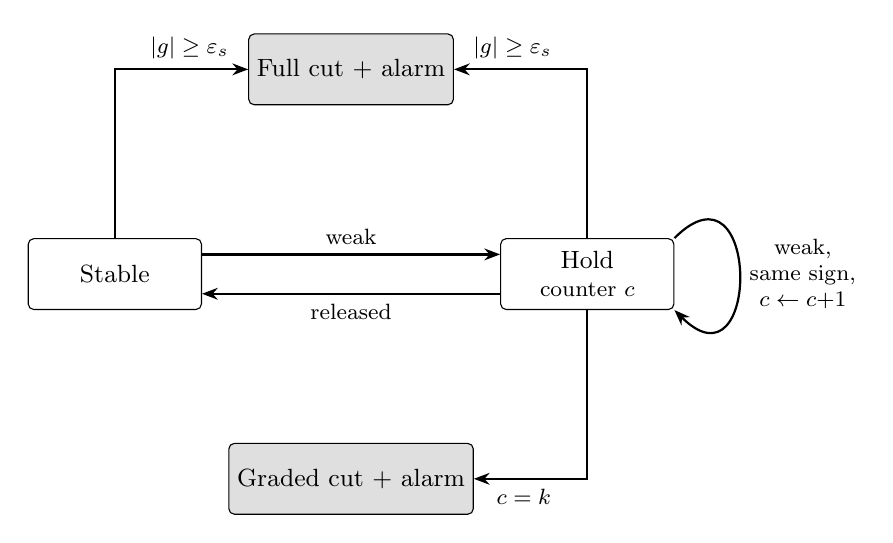
\begin{tikzpicture}[
  st/.style={draw, rounded corners=2pt, align=center, minimum height=9mm, minimum width=2.2cm, inner sep=3pt, font=\small, fill=white},
  ac/.style={draw, rounded corners=2pt, align=center, minimum height=9mm, inner sep=3pt, font=\small, fill=gray!25},
  arr/.style={-{Stealth[length=2mm]}, thick},
  lab/.style={font=\footnotesize, align=center}
]
\node[st] (stable) at (0,0) {Stable};
\node[st] (hold) at (6,0) {Hold\\[-1pt]{\footnotesize counter $c$}};
\node[ac] (full) at (3,2.6) {Full cut + alarm};
\node[ac] (grad) at (3,-2.6) {Graded cut + alarm};
\draw[arr] (stable.north) |- node[lab, pos=0.78, above] {$|g|\ge\varepsilon_s$} (full.west);
\draw[arr] (hold.north) |- node[lab, pos=0.78, above] {$|g|\ge\varepsilon_s$} (full.east);
\draw[arr] ([yshift=2.5mm]stable.east) -- node[lab, above] {weak} ([yshift=2.5mm]hold.west);
\draw[arr] ([yshift=-2.5mm]hold.west) -- node[lab, below] {released} ([yshift=-2.5mm]stable.east);
\draw[arr] (hold.south) |- node[lab, pos=0.78, below] {$c=k$} (grad.east);
\draw[arr] (hold.north east) .. controls +(1.1,1.1) and +(1.1,-1.1) .. node[lab, right, pos=0.5] {weak,\\same sign,\\$c\leftarrow c{+}1$} (hold.south east);
\end{tikzpicture}
\caption{Redrawn state diagram.}
\end{figure}

Read the boxes as the ``moods'' of the detector and the arrows as what makes it change mood.
\begin{itemize}
\item \textbf{Stable} (left): normal state, nothing suspicious.
\item \textbf{Stable $\to$ Full cut} (top left arrow): strong evidence. Cut everything old, raise an alarm.
\item \textbf{Stable $\to$ Hold} (``weak''): weak evidence. Start watching.
\item \textbf{Hold $\to$ Hold} (loop on the right): another weak check in the same direction. Add one to the counter.
\item \textbf{Hold $\to$ Stable} (``released''): the evidence vanished or flipped. Stop watching, reset the counter.
\item \textbf{Hold $\to$ Full cut} (top right arrow): even while holding, strong evidence always wins.
\item \textbf{Hold $\to$ Graded cut} (bottom, ``$c=k$''): weak evidence repeated $k$ times. Partial cut and alarm.
\end{itemize}
The grey boxes are the actions that raise an alarm. After either cut the detector goes back to Stable.

\subsubsection*{Graded cut (Eq.~6)}
How much do we throw away in a graded cut?
\[
\rho=\min\Big(1,\frac{|g|}{\varepsilon_s}\Big).
\]
$\rho$ is the fraction of $W_1$ to drop, counted from the oldest end and rounded to whole buckets. It compares the gap with the strict threshold. A gap just under the strict threshold gives $\rho$ close to 1 (drop almost all of $W_1$). A gap just above the relaxed threshold gives a smaller $\rho$. Because a graded cut only happens after weak evidence, $\rho$ is always at least $\varepsilon_w/\varepsilon_s$.

\emph{Example.} With $\varepsilon_s=0.170$ and a persistent gap of $0.16$: $\rho=0.16/0.17\approx0.94$, so we drop the oldest 94\% of $W_1$. With $\varepsilon_w=0.150$ the smallest possible $\rho$ is $0.150/0.170\approx0.88$. So with these example values, a graded cut always drops most of $W_1$. Choosing $\delta_w$ further from $\delta_s$ widens the weak zone and makes smaller cuts possible. This is why $\delta_w$ is studied in the sensitivity experiments.

\textbf{Why this helps.} A slow change can keep the gap just below the strict threshold for a long time, even though the old data are already out of date. ADWIN-U keeps all that stale data until the gap finally crosses the line. The graded cut removes the stalest part earlier. After a cut, the counter is reset, and for the centroid signal the centroid is reset too.

\subsubsection*{Algorithm 1, line by line}
Algorithm 1 is the same logic written as steps for one check.
\begin{description}[leftmargin=1.8cm, labelwidth=1.6cm]
\item[1, 2] Find the most convincing split and compute the gap $g$ and both thresholds.
\item[3, 4] Strong evidence: drop all of $W_1$, reset $c$, raise an alarm.
\item[5] Otherwise, is it weak evidence?
\item[6, 7] If this is the first weak check ($c=0$) or it points the same way as before, add one to $c$, remember the sign, raise a warning.
\item[8, 9] Otherwise the direction flipped: release ($c=0$).
\item[11 to 14] If $c$ has reached $k$: compute $\rho$, drop that oldest fraction of $W_1$, reset $c$, raise an alarm.
\item[16, 17] No evidence at all: release ($c=0$).
\item[19] No alarm this time.
\end{description}

\emph{A short run with $k=3$.} Check 1: weak, gap positive, $c=1$. Check 2: weak, positive, $c=2$. Check 3: none, released, $c=0$. Check 4: weak, positive, $c=1$. Check 5: weak, positive, $c=2$. Check 6: weak, positive, $c=3=k$, so a graded cut and an alarm. If at check 5 the gap had been strong, there would have been a full cut immediately.

\subsection{Properties and cost (III-F)}

\subsubsection*{ADWIN-U as a special case}
If we set $\delta_w=\delta_s$, both thresholds are equal, the weak zone has zero width, the hold never happens, and our method behaves exactly like ADWIN-U. This makes the comparison clean: any difference must come from the hold and the graded cut.

\subsubsection*{Complexity}
Compared with ADWIN-U we store only one extra counter and one sign and compute one extra threshold. Cuts remove whole buckets, so no extra bookkeeping is needed. So speed and memory should still grow only with $\log|W|$. We will measure this. The centroid signal needs to store one 384-number average, which is a fixed, small cost.

\subsubsection*{False alarms}
The strict threshold comes with a mathematical guarantee that limits false alarms. The graded cut uses the relaxed threshold plus the counter, so that guarantee does not automatically cover it. We are honest about this. That is why we measure false alarms on streams with no change and tune all detectors to the same false-alarm rate before comparing them.

\begin{saybox}{What to say for the Methodology}
``Each document becomes an embedding, the embedding becomes one number, and the number goes into ADWIN's window. ADWIN splits the window into old and new parts and compares their averages. Where ADWIN-U has one threshold and always throws away all the old data, we use two thresholds. Strong evidence gives a full cut. Weak evidence starts a hold with a counter. If weak evidence keeps pointing the same way $k$ times, we throw away only the oldest part, and how much depends on the size of the gap. With equal thresholds we get ADWIN-U back, and the extra cost is one counter.''
\end{saybox}

%====================================================================
\section{Experimental Design, Subsection by Subsection}
\label{sec:exp}

\subsection{Datasets and drift construction (IV-A)}

\subsubsection*{The dataset table (Table~I in the report)}

\begin{center}
\small
\begin{tabular}{>{\raggedright\arraybackslash}p{2.3cm}rl>{\raggedright\arraybackslash}p{4.6cm}l}
\toprule
Dataset & Documents & Classes & Role & Drift truth \\
\midrule
AG News & 127,600 & 4 topics & Abrupt, gradual, recurring drift by topic mix & Known \\
20 Newsgroups & 18,846 & 20 groups & Strong vs.\ subtle drift via macro-topics or sibling groups & Known \\
Amazon reviews & 233.1M & 29 product categories & Real stream in time order (1996 to 2018) & Unknown \\
\bottomrule
\end{tabular}
\end{center}

How to read the columns:
\begin{itemize}
\item \textbf{Documents:} how many texts the dataset has. ``233.1M'' means 233.1 million reviews in the full dataset. We will use a subset of categories.
\item \textbf{Classes:} the categories the texts belong to. We use them to create drift on purpose.
\item \textbf{Role:} what each dataset is used to test.
\item \textbf{Drift truth:} whether we know exactly where the changes are. ``Known'' means we created the changes ourselves. ``Unknown'' means it is real data and nobody knows the exact change points.
\end{itemize}

\subsubsection*{AG News: making different kinds of drift}
AG News has news articles in four topics (World, Sports, Business, Sci/Tech). We build a stream by drawing articles with a chosen \emph{topic mix}, for example 70\% Sports and 30\% World. Then we change the mix:
\begin{itemize}
\item \textbf{Abrupt drift:} at one moment $t_d$ the mix switches completely.
\item \textbf{Gradual drift:} the switch happens smoothly over a period, using the sigmoid in Eq.~7 (below).
\item \textbf{Recurring drift:} after some time the stream goes back to an earlier mix, like a seasonal pattern.
\end{itemize}

\subsubsection*{The sigmoid (Eq.~7)}
\[
p(t)=\frac{1}{1+e^{-4(t-t_d)/w}}
\]
$p(t)$ is the chance that the document at time $t$ comes from the \emph{new} mix. It follows an S-shaped curve: almost 0 long before $t_d$, exactly 0.5 at $t_d$, almost 1 long after. The width $w$ controls how long the transition takes. A small $w$ is almost abrupt and a large $w$ is very gradual.

\emph{Example} with $t_d=5000$ and $w=1000$: at $t=4000$, $p\approx0.02$. At $t=5000$, $p=0.5$. At $t=6000$, $p\approx0.98$.

\subsubsection*{20 Newsgroups: strong vs.\ subtle drift}
20 Newsgroups has posts from 20 discussion groups, which fall into broader families (for example computers, recreation, science, politics).
\begin{itemize}
\item \textbf{Strong drift:} swap groups for groups from a \emph{different} family, for example computer groups for sports groups. The meaning changes a lot.
\item \textbf{Subtle drift:} swap groups for \emph{sibling} groups from the same family, for example PC hardware for Mac hardware. The meaning changes only a little.
\end{itemize}
By changing $w$ and the choice of groups we can test the speed of the drift and its size separately.

\subsubsection*{Drift-free streams}
For each dataset we also build a stream with a fixed mix in random order, so it has no drift. Any alarm on it is a false alarm. We use these streams for tuning (see IV-D).

\subsubsection*{Amazon reviews: the real test}
Amazon reviews sorted by date form a real stream where the drift points are unknown. Since we cannot measure delay without knowing the true change points, we use indirect evidence:
\begin{itemize}
\item the \textbf{alarm rate} (does the detector fire a sensible number of times?),
\item the \textbf{accuracy of a classifier} that is retrained after each alarm, with a limited label budget (do the alarms help in practice?),
\item \textbf{alignment with known events} (do alarms appear near real-world events that we know about?).
\end{itemize}
Together the three datasets cover three kinds of text (news, forum posts, reviews) and both known and unknown drift.

\subsection{Baselines (IV-B)}

Baselines are the methods we compare against. Each one answers a specific ``what if'' question.
\begin{center}
\small
\begin{tabular}{>{\raggedright\arraybackslash}p{4.2cm}>{\raggedright\arraybackslash}p{10.4cm}}
\toprule
Baseline & Why it is included \\
\midrule
ADWIN-U (single and multiple detectors) & Our starting point. We must show we improve on it. \\
Plain ADWIN with several $\delta$ values & Is our gain just the result of picking a better $\delta$? \\
ADWIN with warning and alarm thresholds & Is our gain just the result of having a warning zone, without the hold and graded cut? \\
KSWIN-style test & A popular fixed-window detector, to compare against a non-adaptive window. \\
D3-style detector & A different idea: train a small classifier to tell old from new data. \\
\bottomrule
\end{tabular}
\end{center}
All detectors receive the same signal, so any difference comes from how they handle the window.

\subsection{Evaluation metrics (IV-C)}

First we decide what counts as a ``correct'' alarm. After each real change $t_m$ we allow an \textbf{acceptance window} of length $\Delta_a$. The first alarm inside $[t_m, t_m+\Delta_a]$ is a true detection. Every other alarm is a false alarm. For gradual drift the clock starts at the beginning of the transition.

The three main measures (Eq.~8):
\begin{itemize}
\item \textbf{MTD (mean time to detection):} on average, how many documents after a real change the alarm came. Lower is better.
\item \textbf{FA$_{1k}$ (false alarms per 1,000 documents):} how often the detector cries wolf. Lower is better. Dividing by the stream length lets us compare streams of different lengths.
\item \textbf{MDR (missed-drift rate):} the fraction of real changes that got no alarm at all. Lower is better.
\end{itemize}

\begin{keybox}
\textbf{Worked example.} A stream has $N=20{,}000$ documents and real changes at 5,000, 10,000 and 15,000. The acceptance window is $\Delta_a=1{,}000$. The detector raises alarms at 5,300, 7,200, 10,450 and 18,000.
\begin{itemize}
\item 5,300 is inside $[5000,6000]$: true detection, delay 300.
\item 7,200 is not near any change: false alarm.
\item 10,450 is inside $[10000,11000]$: true detection, delay 450.
\item No alarm in $[15000,16000]$: the change at 15,000 is missed.
\item 18,000: false alarm.
\end{itemize}
So $\mathrm{MTD}=(300+450)/2=375$, $\mathrm{FA}_{1k}=1000\times2/20000=0.1$ and $\mathrm{MDR}=1-2/3\approx0.33$.
\end{keybox}

We also report efficiency: the average window length, the time per document, the peak memory and the throughput (documents per second, which shows the detector keeps up with the stream). BAR, a score from the ADWIN-U paper that combines accuracy with how many labels were requested, is reported as an extra. We do not use accuracy as the main measure, because a benchmark study showed it can reward detectors that simply fire very often.

\subsection{Experimental protocol (IV-D)}

This is the order in which we run the experiments.
\begin{enumerate}
\item \textbf{Calibrate.} On the drift-free streams, tune the main setting of each detector ($\delta$, or $\delta_s$ for ours) until all detectors give the \emph{same} false-alarm rate. Like a race where everyone starts from the same line.
\item \textbf{Repeat.} Run every detector on several random orderings of every drifting stream, so one lucky order cannot decide the result.
\item \textbf{Rank and test.} On each stream, rank the detectors (1st, 2nd, \dots). The \textbf{Friedman test} checks whether the rankings differ by more than chance. If they do, the \textbf{Nemenyi test} tells which pairs of detectors are really different.
\item \textbf{Ablation.} Switch parts of our method on and off to see which part matters:
  \begin{itemize}
  \item \emph{hold only}: persistent weak evidence leads to a full cut instead of a graded cut,
  \item \emph{graded cut without persistence}: $k=1$, so one weak check is enough,
  \item \emph{full policy}: everything on.
  \end{itemize}
\item \textbf{Sensitivity.} Change $\delta_w/\delta_s$ (how wide the weak zone is) and $k$ (how patient the hold is) and see how much the results depend on them.
\item \textbf{Timing.} Embeddings are cached, so the timings only measure the detector.
\end{enumerate}

\begin{saybox}{What to say for the Experimental Design}
``We create drift on purpose in AG News and 20 Newsgroups, so we know exactly where it is, and we vary its type and size. Amazon reviews give a real stream. We compare against ADWIN-U, ADWIN with tuned $\delta$, ADWIN with a warning zone, KSWIN and D3. Every detector is first tuned to the same false-alarm rate, then we measure delay, missed drift, false alarms, time and memory over several random orders and test the rankings statistically. An ablation shows which part of our policy helps.''
\end{saybox}

%====================================================================
\section{Questions the Faculty May Ask}
\label{sec:qa}

\begin{description}[leftmargin=0pt]
\item[Isn't ADWIN already adaptive? What is new?] Yes, ADWIN and ADWIN-U already have an adaptive window and ADWIN-U is already label-free. What is new is the rule for \emph{how much} of the window to drop after evidence of change: hold on weak evidence, and a partial cut when weak evidence persists.
\item[Why not just use a larger $\delta$?] A larger $\delta$ makes the detector faster but also gives more false alarms. Our baselines include ADWIN with a grid of $\delta$ values to check exactly this, and all detectors are compared at the same false-alarm rate.
\item[Isn't the hold just a warning zone?] A warning zone alone only flags. Our hold also checks that the evidence keeps the same direction and then acts with a graded cut. The two-threshold ADWIN baseline and the ablation separate these effects.
\item[Why throw away the oldest part and not a random part?] The oldest data are the most likely to be out of date.
\item[What if kurtosis does not react to topic changes?] That is exactly what contribution (iii) tests. If it does not react, we use the centroid-distance signal.
\item[Why not use accuracy to judge detectors?] A benchmark study (Lukats et al.) showed accuracy can favour detectors that fire often. We use delay, false alarms and missed drift as the main measures.
\item[Do you lose the false-alarm guarantee?] For graded cuts, yes, the strict guarantee does not automatically hold. That is why we measure false alarms directly and calibrate all detectors to the same rate.
\item[Why text only?] Our faculty advised keeping the project focused on text, and text drift has few tested unsupervised methods.
\item[Have you run experiments yet?] Not yet. This report describes the method and the plan. Contribution (ii) is a hypothesis we will test.
\end{description}

%====================================================================
\section{A Two-Minute Script for the Methodology}
\label{sec:script}

\begin{keybox}
``Our input is a text stream with no labels. Each document goes through a frozen MiniLM encoder and becomes 384 numbers, which we cache. Following ADWIN-U, we turn these numbers into one value per document, either kurtosis or skewness. Because we are not sure these react to topic changes, we also use the distance to the average document as a backup.

These values go into ADWIN's window, which is stored in buckets so it stays small. At each check, the window is split into an older and a newer part and we compare their averages. ADWIN-U has one threshold, and when the gap passes it, it throws away the whole old part.

Our policy uses two thresholds. If the gap passes the strict one, we do a full cut, as in ADWIN-U. If it is only above the relaxed one, we hold: we do not cut, we raise a warning and count how many checks in a row point the same way. If the gap disappears or flips, we release the hold. If it persists for $k$ checks, we do a graded cut and drop only the oldest part of the old data, more for a bigger gap. With equal thresholds our method is exactly ADWIN-U, and the extra cost is one counter.

To test it, we inject abrupt, gradual, recurring, strong and subtle drift into AG News and 20 Newsgroups, and use Amazon reviews as a real stream. We tune every detector to the same false-alarm rate and then compare delay, missed drift, false alarms, time and memory against ADWIN-U and other baselines, with statistical tests and an ablation.''
\end{keybox}

\end{document}
